\documentclass[a4paper,12pt]{article}

\usepackage[polish]{babel}
\usepackage[utf8]{inputenc}
\usepackage[T1]{fontenc}
\usepackage[top=2.5cm,bottom=2.5cm,left=3cm,right=3cm]{geometry}
\usepackage{amsmath}
\usepackage{graphicx}
\usepackage{booktabs}
\usepackage{array}
\usepackage{listings}
\usepackage[colorlinks=true, allcolors=blue]{hyperref}
\usepackage{titlesec}

\lstset{
    basicstyle=\ttfamily\small,
    breaklines=true,
    columns=fullflexible
}

\titlespacing*{\subsection}{0pt}{12pt}{6pt}
\setlength{\parindent}{15pt}
\setlength{\parskip}{6pt}

\title{
    \vspace{1.5cm}
    \textbf{PODSTAWY TEORII INFORMACJI}\\
    \vspace{1.5cm}
    Laboratorium 4\\
    Semantyka informacji\\
    \vspace{1.5cm}
    \huge \textbf{Semantyczna ocena użyteczności prognoz meteorologicznych}\\
    \vspace{1cm}
}

\author{
    Maciek Chotkowski \\ Martsin Lazouski \\ Nadia Zięcina \\
    Michał Kasznia \\ Julian Kasiński \\ Volodymyr Kamenchuk \\ Usevalad Nikalaichuk
}

\date{\today}

\begin{document}

\maketitle
\newpage

\tableofcontents
\newpage

\section{Punkt wyjścia projektu}

W folderze projektu znajdują się kolejne etapy pracy laboratoryjnej. Raporty
1 i 2 opisują problem prognoz meteorologicznych oraz stan wiedzy, natomiast
raport 3 przechodzi do poziomu syntaktycznego: dane z różnych źródeł są
pobierane, sprowadzane do plików CSV i oceniane miarami liczbowymi, takimi jak
punkty błędu oraz RMSE.

W etapie 3 analizowane są źródła: Open-Meteo, yr.no, GFS, AIFS i GraphCast.
Dane mają wspólną strukturę:
\begin{verbatim}
nazwa_zrodla/
    temp.csv
    opady.csv
    wiatr.csv
\end{verbatim}

Każdy plik opisuje przebieg jednej wielkości w czasie. Dotychczasowa ocena
odpowiadała więc na pytanie: \textit{czy wartości liczbowe są podobne do
punktu odniesienia?} Raport 4 rozszerza tę analizę o pytanie semantyczne:
\textit{czy prognoza prowadzi do tej samej interpretacji i tej samej decyzji
użytkownika?}

\section{Cel etapu 4}

Celem etapu jest zbudowanie warstwy znaczeniowej nad danymi liczbowymi. Sama
temperatura, suma opadu albo prędkość wiatru nie są jeszcze pełną informacją
dla odbiorcy. Informacją użyteczną jest dopiero interpretacja: czy jest
komfortowo, czy występuje ryzyko opadu, czy wiatr przeszkadza, czy dana
godzina nadaje się do aktywności zewnętrznej.

W tym etapie:
\begin{itemize}
    \item definiujemy profil odbiorcy informacji,
    \item wprowadzamy taksonomię deskryptorów semantycznych,
    \item zamieniamy dane liczbowe na klasy znaczeniowe,
    \item porównujemy modele według zgodności semantycznej,
    \item testujemy wyszukiwanie po treści, a nie po samej wartości liczbowej.
\end{itemize}

\section{Model odbiorcy}

Przyjęto profil użytkownika planującego krótką aktywność zewnętrzną w Warszawie,
np. dojście pieszo, przejazd rowerem, spacer albo organizację niewielkiego
wydarzenia na zewnątrz. Taki użytkownik nie potrzebuje wyłącznie dokładnej
wartości temperatury. Potrzebuje odpowiedzi operacyjnej:
\begin{quote}
Czy w danej godzinie warunki są dobre, wymagają ostrożności, czy są
niekorzystne?
\end{quote}

Dla tego profilu największą wagę mają opady i wiatr, ponieważ bezpośrednio
wpływają na decyzję o wyjściu. Temperatura jest istotna, ale niewielki błąd
temperatury rzadko zmienia decyzję, jeżeli nadal mieści się w tej samej klasie
komfortu.

\section{Taksonomia semantyczna}

Jednostką indeksowania jest jedna godzina prognozy. Obiekt informacyjny ma
atrybuty liczbowe:
\[
    o_t = (T_t, P_t, W_t),
\]
gdzie \(T_t\) oznacza temperaturę, \(P_t\) opad, a \(W_t\) prędkość wiatru.

Na tej podstawie tworzony jest opis znaczeniowy:
\[
    d_t = (c_T, c_P, c_W, c_D),
\]
gdzie \(c_T\), \(c_P\), \(c_W\) są deskryptorami temperatury, opadu i wiatru,
a \(c_D\) jest końcową klasą decyzyjną.

\begin{table}[h]
\centering
\caption{Przyjęte deskryptory semantyczne}
\begin{tabular}{lll}
\toprule
Cecha & Zakres liczbowy & Deskryptor \\
\midrule
Temperatura & \(T < 0^\circ C\) & mróz \\
Temperatura & \(0 \leq T < 10^\circ C\) & zimno \\
Temperatura & \(10 \leq T < 18^\circ C\) & chłodno \\
Temperatura & \(18 \leq T < 25^\circ C\) & komfort \\
Temperatura & \(25 \leq T < 30^\circ C\) & ciepło \\
Temperatura & \(T \geq 30^\circ C\) & upał \\
\midrule
Opad & \(P \leq 0.1\) mm & brak opadu \\
Opad & \(0.1 < P \leq 0.5\) mm & słaby opad \\
Opad & \(0.5 < P \leq 2.0\) mm & umiarkowany opad \\
Opad & \(P > 2.0\) mm & silny opad \\
\midrule
Wiatr & \(W < 2.0\) m/s & cisza \\
Wiatr & \(2.0 \leq W < 5.0\) m/s & lekki wiatr \\
Wiatr & \(5.0 \leq W < 8.0\) m/s & wietrznie \\
Wiatr & \(W \geq 8.0\) m/s & silny wiatr \\
\bottomrule
\end{tabular}
\end{table}

Końcowa klasa decyzyjna ma trzy wartości: \textit{dobre}, \textit{ostrożnie}
i \textit{złe}. Warunki są oznaczane jako złe przy umiarkowanym lub silnym
opadzie, silnym wietrze, mrozie albo upale. Klasa ostrożnie oznacza sytuacje
graniczne: zimno, słaby opad albo wiatr odczuwalny.

Ten etap jest realizowany w kodzie przez funkcje mapujące wartości liczbowe na
deskryptory. Poniżej wklejono najważniejszy fragment z pliku
\texttt{semantic\_weather\_common.py}. Kod pokazuje, że model nie operuje już
wyłącznie na liczbach, ale zamienia je na znaczenia używane później w decyzji.

\begin{lstlisting}[language=Python]
def temp_label(value):
    if value < 0:
        return "mroz"
    if value < 10:
        return "zimno"
    if value < 18:
        return "chlodno"
    if value < 25:
        return "komfort"
    if value < 30:
        return "cieplo"
    return "upal"

def decision_label(temp, rain, wind):
    if temp in {"mroz", "upal"} or rain in {"umiarkowany_opad", "silny_opad"}:
        return "zle"
    if wind == "silny_wiatr":
        return "zle"
    if temp in {"zimno"} or rain == "slaby_opad" or wind == "wietrznie":
        return "ostroznie"
    return "dobre"
\end{lstlisting}

\section{Miary oceny semantycznej}

Miara syntaktyczna karze każdy błąd liczbowy. Miara semantyczna karze przede
wszystkim zmianę znaczenia. Przykładowo różnica temperatury z \(19^\circ C\)
na \(20^\circ C\) jest błędem liczbowym, ale nie zmienia interpretacji
użytkownika. Różnica z \(17.8^\circ C\) na \(18.2^\circ C\) może natomiast
zmienić klasę z chłodno na komfort.

Dla każdej godziny obliczono ważoną zgodność semantyczną:
\[
S = 1 - (0.25 d_T + 0.45 d_P + 0.30 d_W),
\]
gdzie \(d_T\), \(d_P\), \(d_W\) są znormalizowanymi odległościami między
klasami temperatury, opadu i wiatru. Waga opadu jest największa, ponieważ dla
przyjętego użytkownika opad najsilniej wpływa na decyzję.

Dodatkowo liczono:
\begin{itemize}
    \item zgodność końcowej decyzji użytkownika,
    \item zgodność klas temperatury, opadu i wiatru,
    \item precyzję, przywołanie, F1 i stopę sukcesu dla zapytań semantycznych.
\end{itemize}

\section{Punkty krytyczne informacji}

Po pierwszej wersji analizy metoda została zmieniona. Sama zgodność klas
semantycznych okazała się niewystarczająca, ponieważ niektóre punkty danych są
ważniejsze od pozostałych. W prognozie pogody istnieją granice, przy których
niewielki błąd liczbowy powoduje dużą zmianę znaczenia informacji. Przykładem
jest temperatura \(-0.6^\circ C\) i prognoza \(0.6^\circ C\). Różnica wynosi
tylko \(1.2^\circ C\), ale po jednej stronie granicy możliwy jest śnieg,
zamarzanie wody albo oblodzenie, a po drugiej stronie użytkownik może
interpretować sytuację jako zwykły deszcz lub brak ryzyka zamarzania.

Z tego powodu do analizy dodano osobną warstwę punktów krytycznych. Nie są to
zwykłe błędy numeryczne, lecz miejsca, w których zmienia się sens komunikatu
dla odbiorcy.

\begin{table}[h]
\centering
\caption{Punkty krytyczne dodane do analizy}
\begin{tabular}{lll}
\toprule
Punkt krytyczny & Warunek & Znaczenie dla użytkownika \\
\midrule
Granica zamarzania & \(T \leq 0^\circ C\) & ryzyko lodu, śniegu, śliskiej nawierzchni \\
Opad przy 0°C & \(T \leq 0.5^\circ C\) i \(P > 0.1\) & możliwy śnieg lub marznący opad \\
Opad istotny & \(P > 0.5\) mm & zmiana decyzji o aktywności zewnętrznej \\
Silny opad & \(P > 2.0\) mm & warunki niekorzystne \\
Silny wiatr & \(W \geq 8.0\) m/s & ryzyko dyskomfortu i ograniczeń bezpieczeństwa \\
Temperatura skrajna & \(T \leq -5^\circ C\) lub \(T \geq 30^\circ C\) & ryzyko wychłodzenia albo przegrzania \\
\bottomrule
\end{tabular}
\end{table}

Dla każdego modelu sprawdzane jest, czy wykrywa tę samą stronę progu
krytycznego co punkt odniesienia. Jeżeli punkt odniesienia wskazuje mróz, a
model pokazuje temperaturę dodatnią, taki przypadek otrzymuje większą wagę
interpretacyjną niż zwykła różnica temperatur wewnątrz tej samej klasy.

Kod tego etapu znajduje się również w pliku
\texttt{semantic\_weather\_common.py}. Fragment poniżej pokazuje, jakie
sytuacje są traktowane jako punkty krytyczne. Nie jest to pełny model prognozy,
tylko dodatkowa warstwa kontroli znaczenia wyniku.

\begin{lstlisting}[language=Python]
def critical_flags(df, source_key):
    temp = df[f"temp_{source_key}"]
    rain = df[f"opady_{source_key}"]
    wind = df[f"wiatr_{source_key}"]

    return pd.DataFrame({
        "freezing_boundary": temp <= 0.0,
        "snow_or_ice_risk": (temp <= 0.5) & (rain > 0.1),
        "significant_precipitation": rain > 0.5,
        "heavy_precipitation": rain > 2.0,
        "strong_wind": wind >= 8.0,
        "thermal_extreme": (temp <= -5.0) | (temp >= 30.0),
    }, index=df.index)
\end{lstlisting}

\section{Własny algorytm przewidywania pogody}

Właściwym celem tej części projektu nie jest tylko porównanie gotowych modeli,
ale zbudowanie własnego algorytmu prognozowania. Dlatego analiza została
rozszerzona o model autorski, który łączy kilka źródeł prognozy i dopasowuje
ich znaczenie do danych referencyjnych oraz punktów krytycznych.

Zaproponowany algorytm można nazwać krytycznie ważonym modelem zespołowym.
Nie wybiera on jednego najlepszego źródła, lecz tworzy prognozę jako ważoną
kombinację kilku modeli:
\[
\hat{x}_m(t) = \sum_i w_{i,m} x_{i,m}(t),
\]
gdzie \(x_{i,m}(t)\) oznacza prognozę źródła \(i\) dla zmiennej \(m\), a
\(w_{i,m}\) jest wagą tego źródła dla temperatury, opadów albo wiatru.

Wagi nie są takie same dla wszystkich wielkości. Model może ufać jednemu
źródłu bardziej przy temperaturze, a innemu przy opadach albo wietrze. Dzięki
temu algorytm jest bardziej elastyczny niż zwykła średnia arytmetyczna.

\subsection{Kroki algorytmu}

Algorytm działa w następujących krokach:
\begin{enumerate}
    \item wczytuje prognozy AIFS, GraphCast, Open-Meteo, yr.no i GFS,
    \item wyrównuje dane po czasie, aby każda godzina miała komplet wartości,
    \item dzieli dane na część dopasowania i część testową,
    \item dla każdego źródła liczy błąd ważony krytycznie,
    \item zamienia błędy na wagi modelu,
    \item wyznacza prognozę jako średnią ważoną,
    \item wykonuje korektę przy progach krytycznych, np. \(0^\circ C\), opadzie istotnym i silnym wietrze,
    \item zapisuje wynik jako nowe źródło danych: \texttt{own\_model}.
\end{enumerate}

Błąd używany do dopasowania ma postać:
\[
E_{i,m} = \frac{1}{n}\sum_t \left(|x_{ref,m}(t)-x_{i,m}(t)| + P_{crit}(t)\right),
\]
gdzie \(P_{crit}(t)\) jest dodatkową karą za pomyłkę po niewłaściwej stronie
progu krytycznego. Przykładowo model jest karany mocniej, jeżeli punkt
odniesienia pokazuje temperaturę poniżej \(0^\circ C\), a prognoza pokazuje
temperaturę dodatnią.

Wagi wyznaczane są ze wzoru:
\[
w_{i,m} \sim \frac{1}{(E_{i,m}+0.25)^2}.
\]
Dodano również ograniczenie maksymalnej wagi jednego źródła do 45\%. Jest to
ważne, ponieważ w obecnych danych Open-Meteo jest bardzo bliskie punktowi
odniesienia i bez ograniczenia mogłoby zdominować cały model. Nasz algorytm
ma być własną prognozą zespołową, a nie kopią jednego źródła.

Poniższy fragment kodu pochodzi z pliku \texttt{own\_weather\_model.py}. To
jest właściwy fragment uczenia naszego modelu: najpierw liczony jest błąd
ważony krytycznie, potem błąd jest zamieniany na wagę. Im mniejszy błąd źródła,
tym większy jego udział w końcowej prognozie.

\begin{lstlisting}[language=Python]
def learn_weights(frame, metric, train_size):
    train = frame.iloc[:train_size]
    actual = train[f"{metric}_ground_truth"]
    raw_weights = {}

    for source in MODEL_SOURCES:
        column = f"{metric}_{source.key}"
        if column not in train.columns:
            continue
        error = critical_weighted_error(metric, actual, train[column])
        raw_weights[source.key] = 1.0 / ((error + 0.25) ** 2)

    return cap_and_normalize(raw_weights)
\end{lstlisting}

Kolejny fragment pokazuje samo tworzenie prognozy. Dla każdej godziny model
mnoży prognozę danego źródła przez dopasowaną wagę, sumuje wkłady i otrzymuje
nową wartość naszej prognozy.

\begin{lstlisting}[language=Python]
def predict_metric(frame, metric, weights):
    prediction = pd.Series(0.0, index=frame.index)
    used_weight = 0.0

    for source_key, weight in weights.items():
        column = f"{metric}_{source_key}"
        if column in frame.columns:
            prediction += frame[column] * weight
            used_weight += weight

    prediction = prediction / used_weight
    if METRICS[metric]["min_value"] is not None:
        prediction = prediction.clip(lower=METRICS[metric]["min_value"])
    return prediction
\end{lstlisting}

Ostatni fragment z tego etapu pokazuje korektę przy progach krytycznych.
Przykładowo, jeżeli prognoza jest bardzo blisko \(0^\circ C\), występuje opad,
a wystarczająco dużo źródeł wskazuje temperaturę ujemną, model przesuwa wynik
na stronę mrozu. Chodzi o to, aby nie zgubić znaczenia sytuacji granicznej.

\begin{lstlisting}[language=Python]
if abs(corrected["temp"]) <= 0.8 and corrected["opady"] > 0.1:
    freezing_weight = sum(
        weights["temp"].get(source.key, 0.0)
        for source in MODEL_SOURCES
        if row[f"temp_{source.key}"] <= 0.0
    )
    if freezing_weight >= 0.40:
        corrected["temp"] = min(corrected["temp"], -0.1)
    else:
        corrected["temp"] = max(corrected["temp"], 0.1)
\end{lstlisting}

\subsection{Dopasowanie modelu}

Model dopasowano na pierwszych 35 godzinach wspólnego zakresu danych, a
ostatnie 16 godzin zostawiono jako prosty test. Dopasowanie polegało na
wyznaczeniu wag osobno dla temperatury, opadów i wiatru.

\begin{table}[h]
\centering
\caption{Wagi źródeł po dopasowaniu własnego modelu}
\begin{tabular}{lrrr}
\toprule
Źródło & Temperatura & Opady & Wiatr \\
\midrule
AIFS & 0.167 & 0.201 & 0.127 \\
GraphCast & 0.036 & 0.015 & 0.012 \\
Open-Meteo & 0.450 & 0.265 & 0.450 \\
yr.no & 0.142 & 0.265 & 0.158 \\
GFS & 0.205 & 0.254 & 0.254 \\
\bottomrule
\end{tabular}
\end{table}

Po dopasowaniu model zapisał trzy pliki wynikowe:
\begin{verbatim}
raport4/own_model/temp.csv
raport4/own_model/opady.csv
raport4/own_model/wiatr.csv
\end{verbatim}

W części testowej uzyskano następujące wyniki:
\begin{table}[h]
\centering
\caption{Wyniki testowe własnego modelu}
\begin{tabular}{lrrr}
\toprule
Zmienna & MAE & RMSE & Błąd krytycznie ważony \\
\midrule
Temperatura & 1.593 & 1.709 & 1.593 \\
Opady & 0.011 & 0.014 & 0.011 \\
Wiatr & 0.306 & 0.360 & 0.306 \\
\bottomrule
\end{tabular}
\end{table}

Zgodność decyzji użytkownika w części testowej wyniosła 100\%. Trzeba jednak
pamiętać, że obecne okno danych jest łatwe pogodowo: nie zawiera mrozu, silnego
opadu ani silnego wiatru. Dlatego najważniejszym elementem modelu nie jest
sam wynik testu, lecz mechanizm dopasowania wag i dodatkowe kary za błędy przy
progach krytycznych.

\section{Implementacja}

Dla etapu 4 przygotowano pięć plików kodu:
\begin{itemize}
    \item \texttt{semantic\_weather\_common.py} -- konfiguracja źródeł, wczytywanie CSV, mapowanie wartości na deskryptory i funkcje metryk,
    \item \texttt{semantic\_evaluation.py} -- ranking semantyczny modeli oraz wykresy,
    \item \texttt{semantic\_search\_tests.py} -- testy wyszukiwania po treści: precyzja, przywołanie, F1 i stopa sukcesu,
    \item \texttt{own\_weather\_model.py} -- własny algorytm prognozowania pogody i dopasowanie wag,
    \item \texttt{critical\_scenario\_analysis.py} -- scenariusze pokazujące znaczenie progów krytycznych.
\end{itemize}

Kod wczytuje dane z folderu \texttt{raport\_3}. Ponieważ część plików CSV w
repozytorium zawiera aktualnie znaczniki konfliktów git, moduł wczytujący
pomija linie zaczynające się od \texttt{<<<<<<<}, \texttt{=======} i
\texttt{>>>>>>>}. Nie zmienia to danych źródłowych, ale pozwala wykonać
analizę mimo niezamkniętego konfliktu.

Najważniejsze fragmenty kodu zostały wklejone bezpośrednio przy etapach, których
dotyczą. Pełne wersje skryptów znajdują się w folderze \texttt{raport4}.

\section{Wyniki rankingu semantycznego}

Analiza została wykonana dla 51 wspólnych godzin. Punktem odniesienia jest
katalog \texttt{default\_model}, tak jak w raporcie 3. Należy pamiętać, że
Open-Meteo osiąga wynik 100\%, ponieważ w obecnym zestawie danych jest
praktycznie tożsame z przyjętym punktem odniesienia. Ten wynik służy jako test
poprawności procedury, a nie jako niezależny dowód przewagi modelu.

\begin{table}[h]
\centering
\caption{Ranking zgodności semantycznej}
\begin{tabular}{lrrrr}
\toprule
Model & Godziny & Zgodność sem. [\%] & Zgodność decyzji [\%] & Opad [\%] \\
\midrule
Open-Meteo & 51 & 100.0 & 100.0 & 100.0 \\
Nasz model & 51 & 96.9 & 100.0 & 100.0 \\
GFS & 51 & 95.8 & 100.0 & 100.0 \\
AIFS & 51 & 95.2 & 100.0 & 100.0 \\
Yr.no & 51 & 94.2 & 92.2 & 100.0 \\
GraphCast & 51 & 82.3 & 15.7 & 64.7 \\
\bottomrule
\end{tabular}
\end{table}

\begin{figure}[h]
\centering
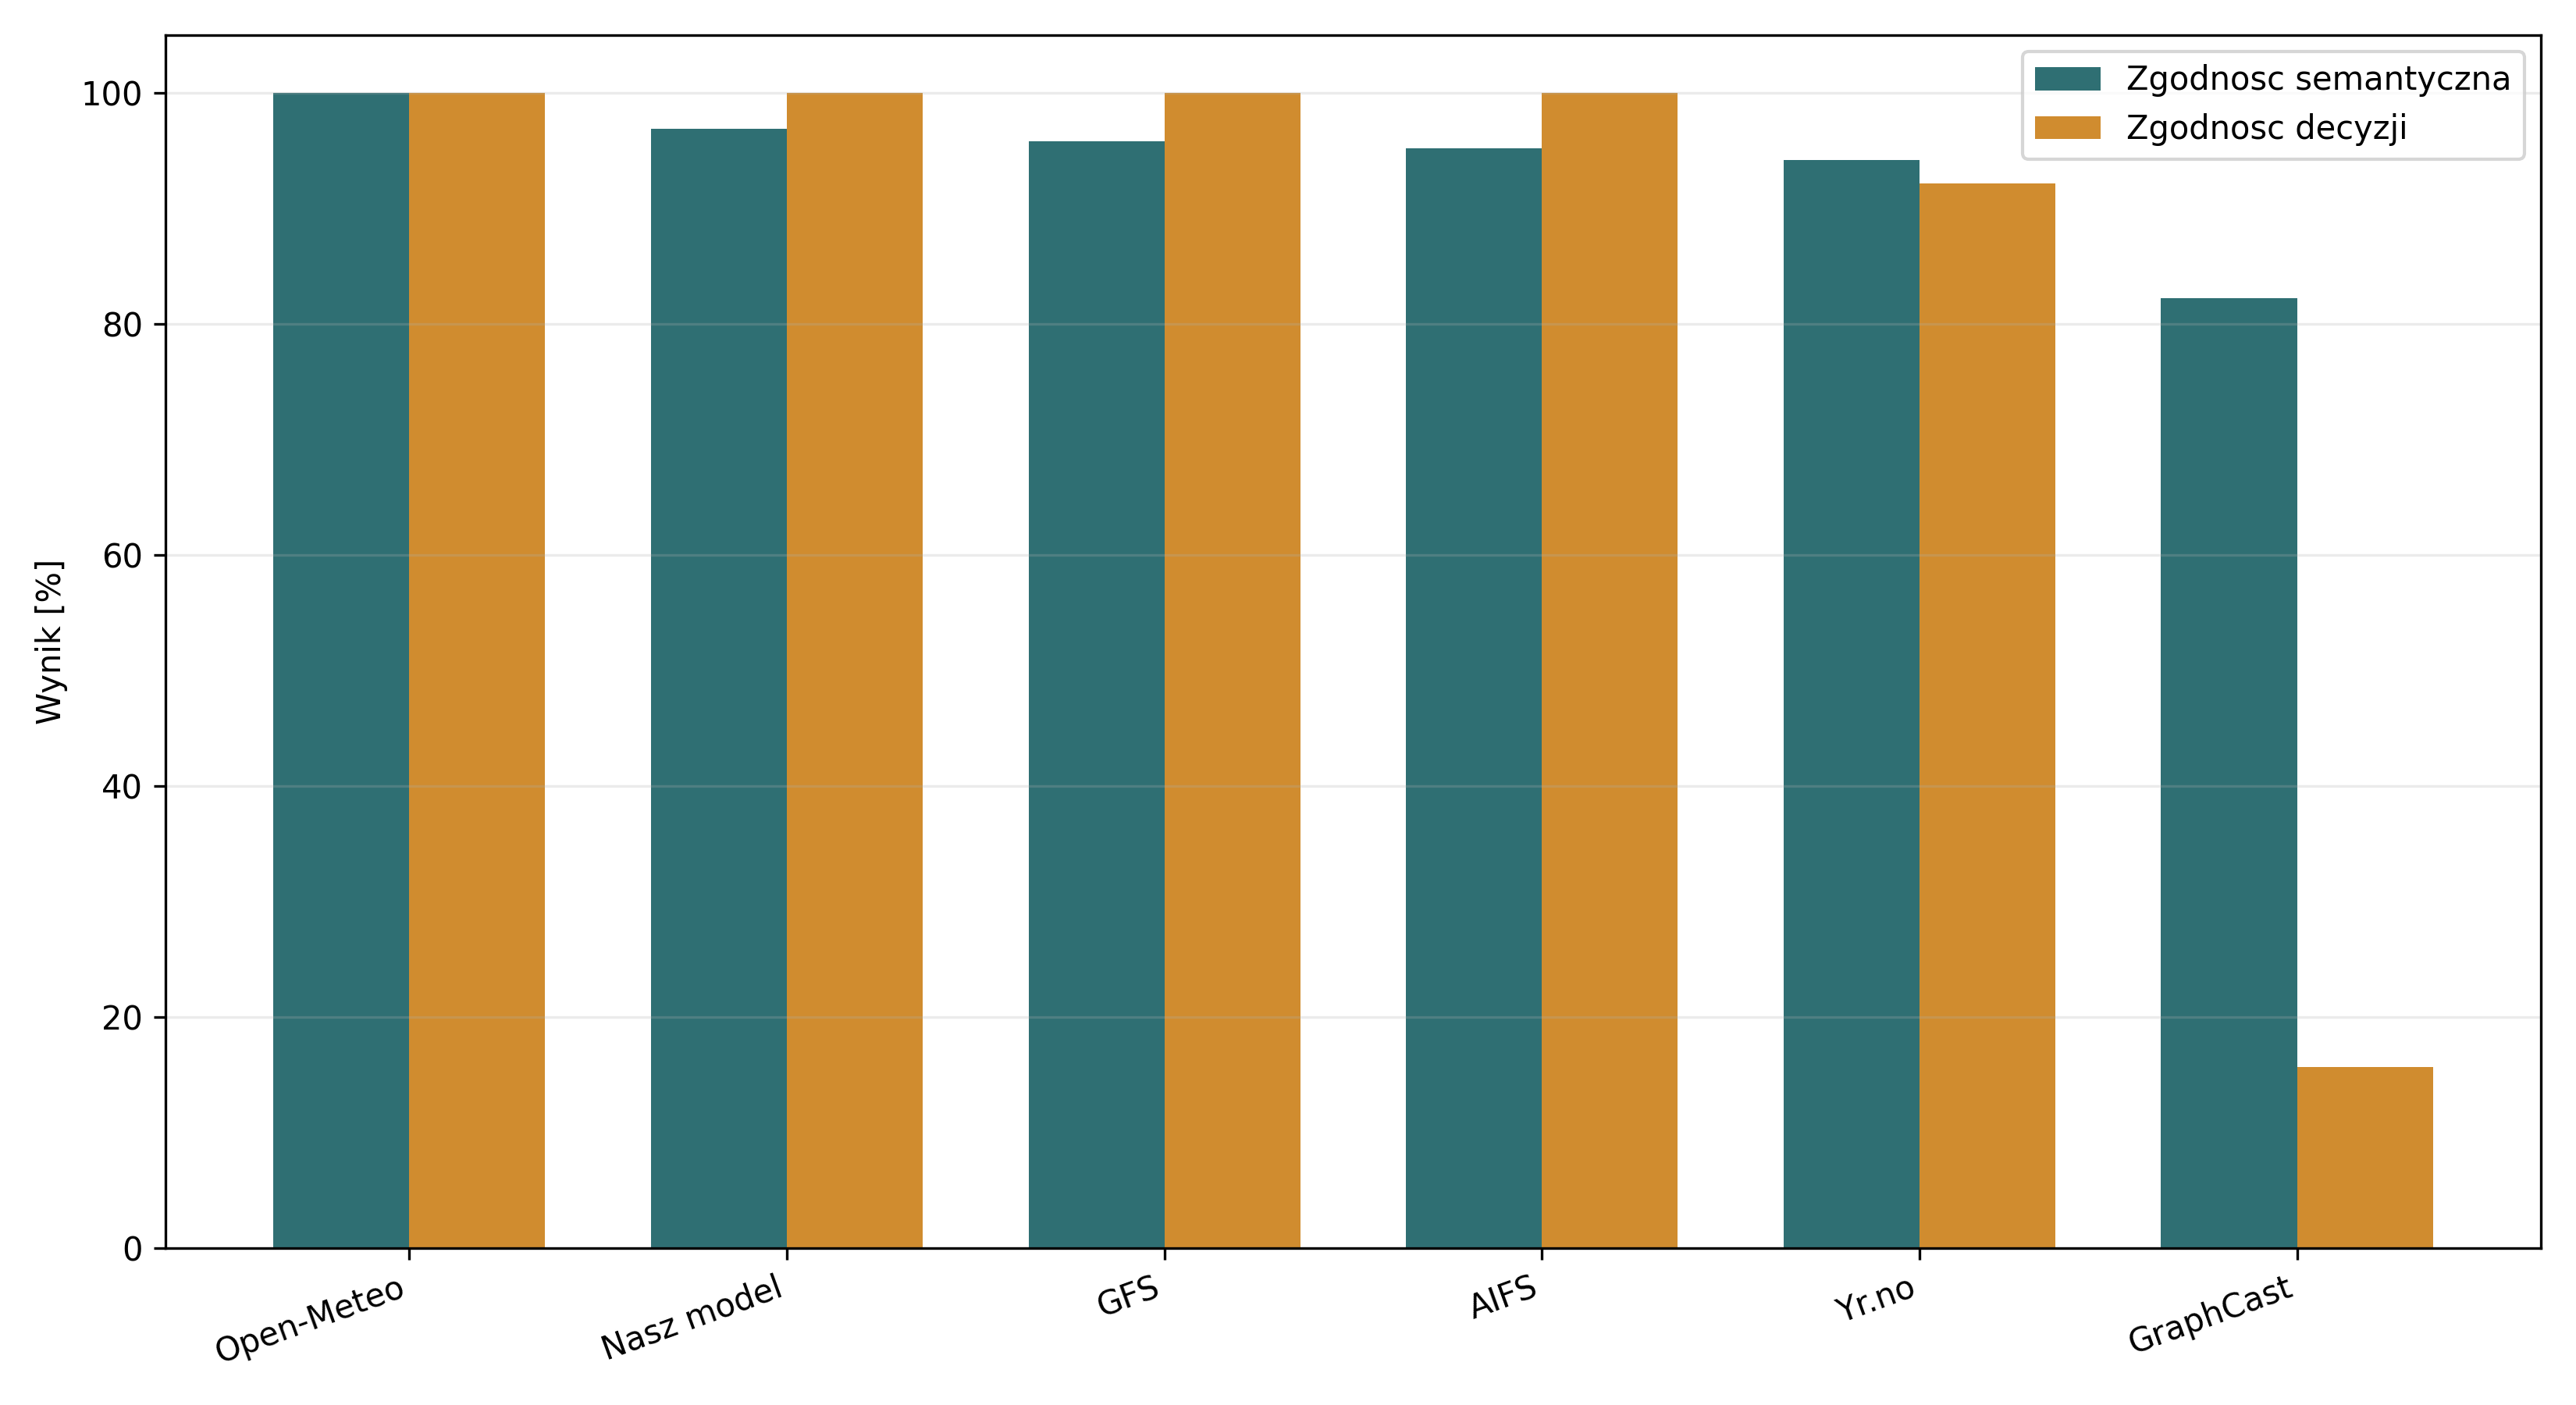
\includegraphics[width=\textwidth]{semantic_decision_accuracy.png}
\caption{Porównanie zgodności semantycznej i zgodności decyzji użytkownika.}
\end{figure}

Wyniki pokazują, że nasz model uzyskał najwyższą zgodność semantyczną spośród
modeli, które nie są bezpośrednim punktem odniesienia. Jest to efekt ważenia
źródeł oraz ograniczenia wpływu słabszych prognoz. Modele GFS i AIFS również
mogą mieć błędy wartości liczbowych, ale w badanym oknie czasowym nie zmieniają
one końcowej decyzji użytkownika. GraphCast wypada gorzej, ponieważ częściej
przechodzi do innych klas temperatury, opadu lub wiatru, co silnie obniża
zgodność decyzji.

\begin{figure}[h]
\centering
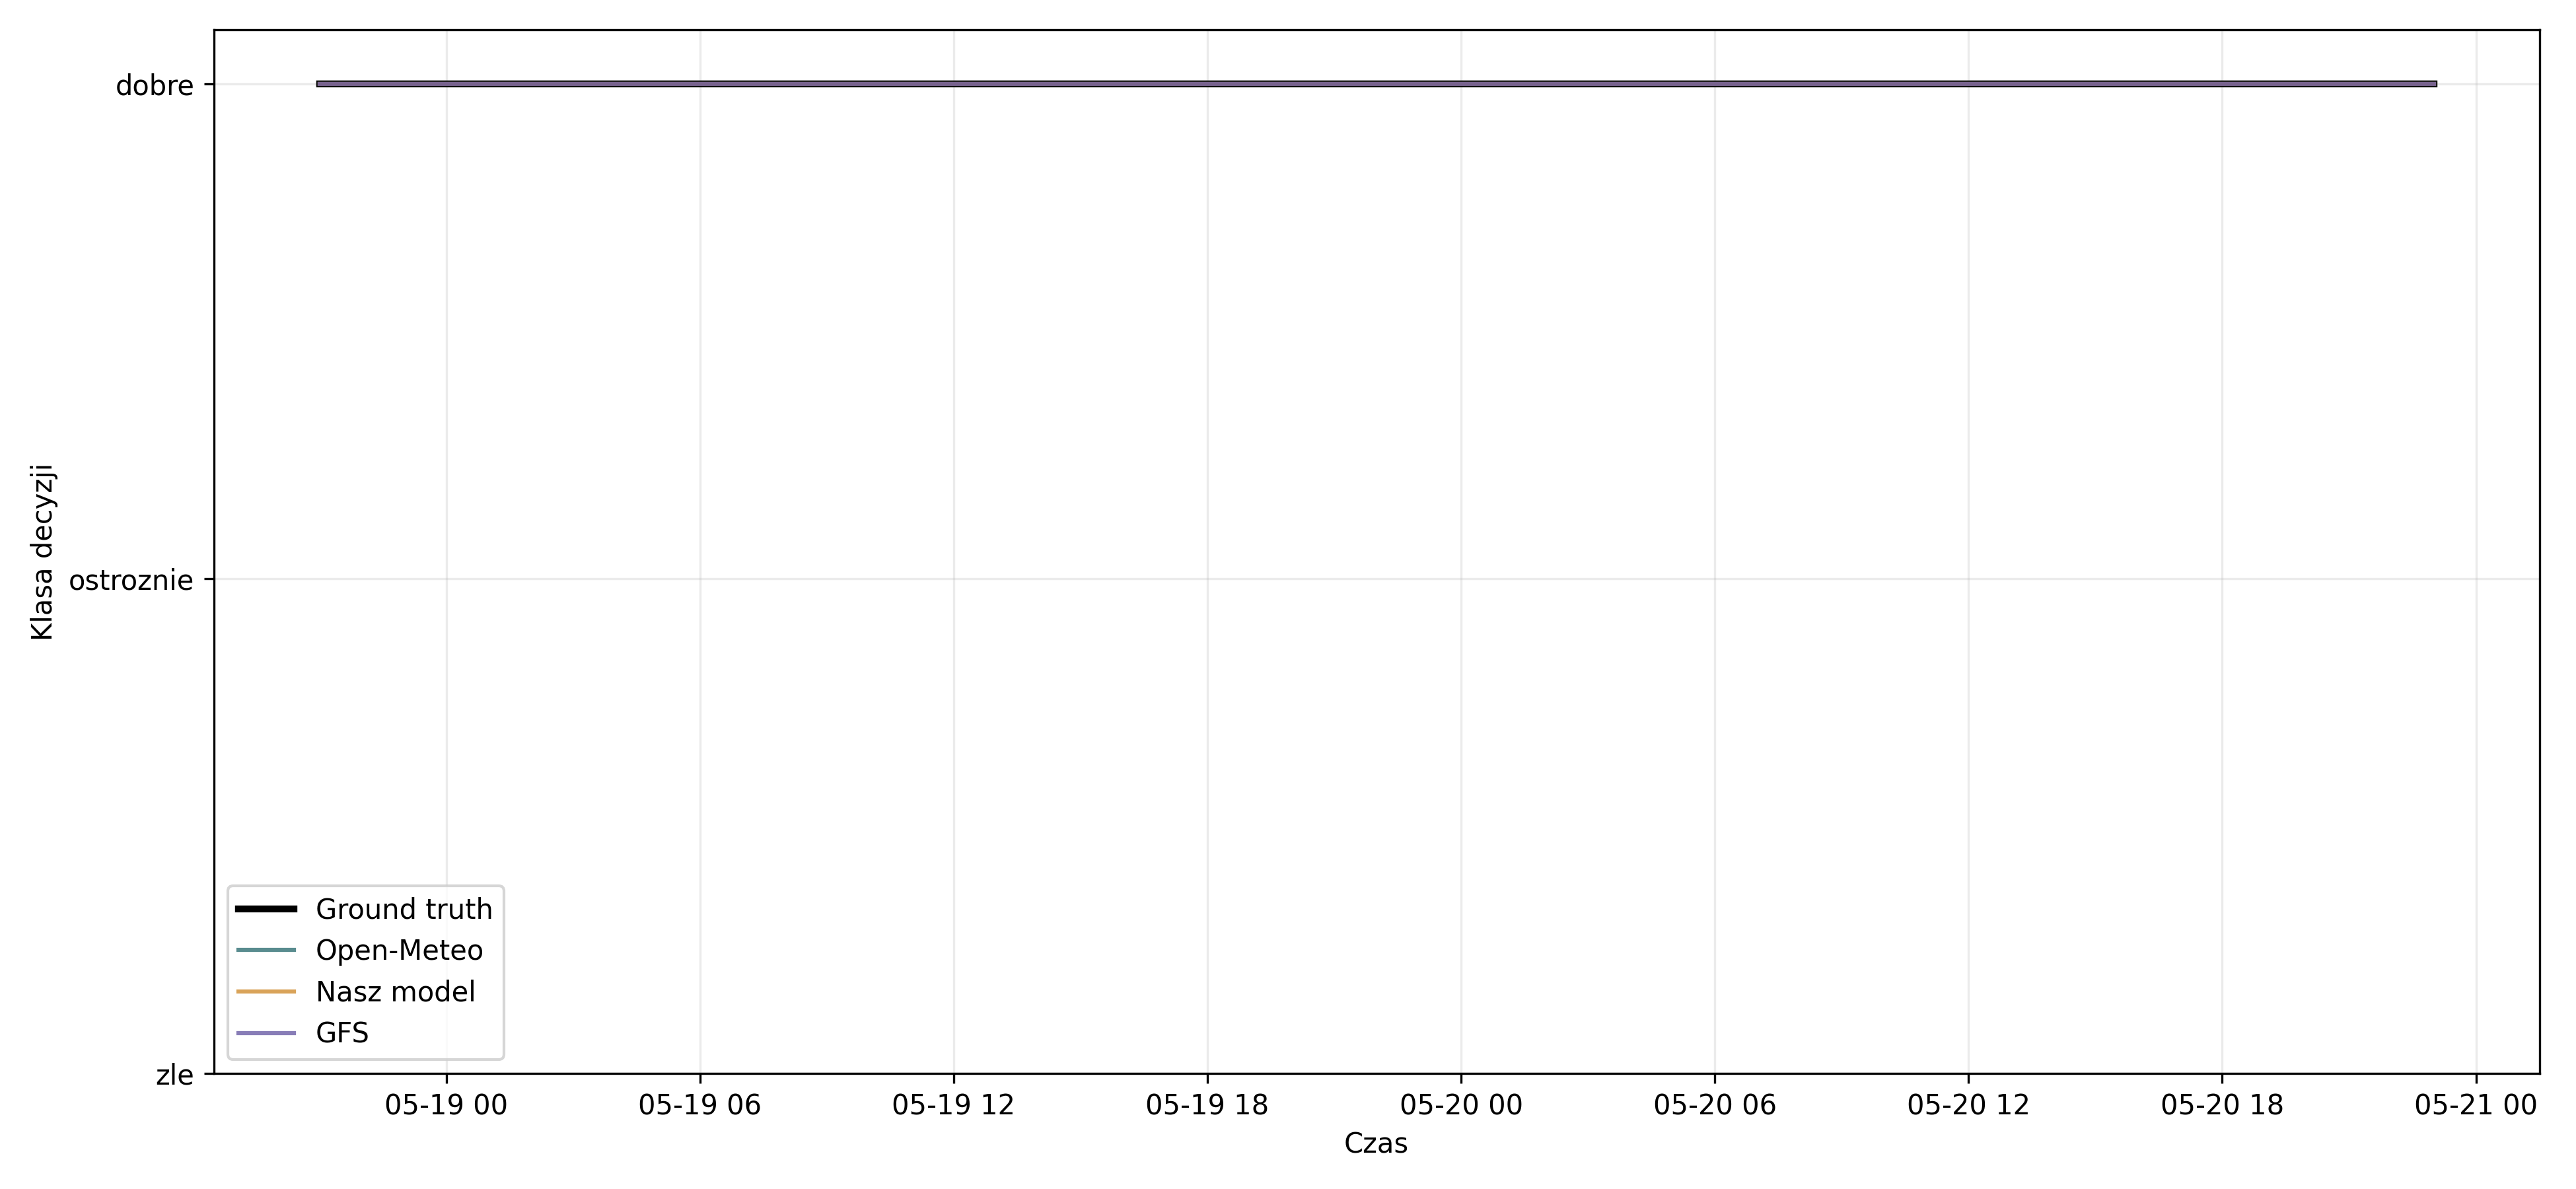
\includegraphics[width=\textwidth]{semantic_timeline.png}
\caption{Przebieg klas decyzyjnych w czasie dla punktu odniesienia i najlepszych modeli.}
\end{figure}

\section{Analiza punktów krytycznych}

Po rozszerzeniu metody przeliczono osobny raport
\texttt{critical\_points\_summary.csv}. W aktualnym zbiorze 51 wspólnych godzin
nie wystąpiły przypadki referencyjne przekraczające progi krytyczne:
temperatura nie przechodziła przez \(0^\circ C\), nie było opadu przy
temperaturze bliskiej zera, istotnych opadów, silnego wiatru ani temperatur
skrajnych. Z tego powodu wszystkie modele mają w tej konkretnej próbce
\(0\) błędów krytycznych.

Ten wynik nie oznacza jednak, że progi krytyczne są zbędne. Oznacza tylko, że
badane okno danych było pogodowo łatwe. Dlatego dodano również analizę
scenariuszową, w której sprawdzono typowe przypadki graniczne.

\begin{table}[h]
\centering
\caption{Scenariusze pokazujące znaczenie progów krytycznych}
\begin{tabular}{p{4.2cm}rrrrp{4.1cm}}
\toprule
Scenariusz & \(T_{ref}\) & \(T_m\) & \(P_{ref}\) & \(P_m\) & Zmiana decyzji & Znaczenie \\
\midrule
Granica zamarzania i możliwy śnieg & -0.6 & 0.6 & 0.4 & 0.4 & tak & możliwa zmiana: śnieg/lód zamiast deszczu \\
Pominięty opad istotny & 3.0 & 3.2 & 0.8 & 0.1 & tak & model nie ostrzega przed opadem zmieniającym decyzję \\
Fałszywy alarm opadowy & 7.0 & 7.1 & 0.0 & 0.7 & tak & model odrzuca dobre okno czasowe \\
Granica silnego wiatru & 16.0 & 16.0 & 0.0 & 0.0 & tak & mały błąd wiatru zmienia ocenę bezpieczeństwa \\
Próg upału & 30.2 & 29.4 & 0.0 & 0.0 & tak & mała różnica ukrywa ryzyko przegrzania \\
Próg mrozu silniejszego & -5.3 & -4.7 & 0.0 & 0.0 & nie & decyzja zostaje zła, ale zmienia się poziom ryzyka \\
\bottomrule
\end{tabular}
\end{table}

Scenariusze pokazują, że błąd o podobnej wartości liczbowej może mieć zupełnie
inny ciężar informacyjny. Różnica \(1^\circ C\) przy temperaturach dodatnich
często jest mało istotna, ale różnica wokół \(0^\circ C\) może zmienić rodzaj
opadu, ocenę bezpieczeństwa i zalecenie dla użytkownika. W finalnej wersji
metody takie przypadki powinny być traktowane jako błędy semantycznie cięższe
niż zwykłe przesunięcie wewnątrz tej samej klasy.

\section{Testy wyszukiwania semantycznego}

Na danych zbudowano prosty indeks treści. Zamiast pytać o wartości liczbowe,
można zadawać zapytania dotyczące znaczenia:
\begin{itemize}
    \item Q1: dobre okno na aktywność zewnętrzną,
    \item Q2: ryzyko opadów istotnych,
    \item Q3: ryzyko wiatru dla użytkownika,
    \item Q4: warunki niekorzystne,
    \item Q5: komfort termiczny.
\end{itemize}

Dla każdego modelu porównano zbiór godzin zwróconych przez zapytanie ze zbiorem
godzin referencyjnych. Obliczono precyzję, przywołanie, F1 oraz stopę sukcesu.

Ten etap ma również własny fragment kodu w pliku
\texttt{semantic\_search\_tests.py}. Poniżej pokazano ideę zapytań: zapytanie
nie wybiera godzin po surowej temperaturze lub opadzie, tylko po wcześniej
nadanych deskryptorach i decyzjach.

\begin{lstlisting}[language=Python]
def query_good_outdoor(df, key):
    return df[f"decision_{key}"] == "dobre"

def query_rain_risk(df, key):
    return df[f"rain_label_{key}"].isin(
        ["umiarkowany_opad", "silny_opad"]
    )

SEARCH_QUERIES = [
    ("Q1", "dobre okno na aktywnosc zewnetrzna", query_good_outdoor),
    ("Q2", "ryzyko opadow istotnych", query_rain_risk),
]
\end{lstlisting}

\begin{table}[h]
\centering
\caption{Wybrane wyniki testów wyszukiwania}
\begin{tabular}{lrrr}
\toprule
Model & Q1 F1 [\%] & Q5 F1 [\%] & Q3 stopa sukcesu [\%] \\
\midrule
Open-Meteo & 100.0 & 100.0 & 100.0 \\
GFS & 100.0 & 100.0 & 100.0 \\
AIFS & 100.0 & 100.0 & 100.0 \\
Nasz model & 100.0 & 100.0 & 100.0 \\
Yr.no & 95.9 & 95.9 & 100.0 \\
GraphCast & 27.1 & 67.5 & 80.4 \\
\bottomrule
\end{tabular}
\end{table}

W badanym zakresie nie wystąpiły referencyjne godziny z istotnym opadem ani
złymi warunkami. Z tego powodu precyzja i przywołanie dla zapytań Q2 i Q4 nie
są diagnostyczne: brak trafień może oznaczać poprawne zachowanie systemu, ale
nie sprawdza zdolności wykrywania realnych zdarzeń niekorzystnych. Ten etap
wskazuje więc potrzebę rozszerzenia zbioru testowego o okresy z opadami,
silnym wiatrem i skrajnymi temperaturami.

\section{Ocena przydatności i ograniczenia}

Warstwa semantyczna poprawia interpretowalność systemu. Użytkownik nie musi
analizować tabel temperatur, opadów i wiatru, ponieważ otrzymuje klasy
znaczeniowe oraz końcową decyzję. Jest to zgodne z celem etapu 4: uzyskać
reprezentatywny opis istoty informacji w konkretnym zastosowaniu.

Najważniejsze ograniczenia:
\begin{itemize}
    \item punkt odniesienia nie jest niezależną stacją pomiarową, lecz jednym z modeli,
    \item zakres danych obejmuje tylko 51 wspólnych godzin,
    \item w danych brakuje trudnych przypadków pogodowych,
    \item progi semantyczne są eksperckie i powinny być dopasowane do realnych opinii użytkowników.
\end{itemize}

\section{Wnioski}

Raport 4 pokazuje przejście od analizy syntaktycznej do semantycznej. W
raporcie 3 model był oceniany głównie przez odległość liczbową od punktu
odniesienia. W tym etapie oceniamy, czy model zachowuje znaczenie informacji:
czy wskazuje te same klasy pogody, te same okna czasowe i tę samą decyzję
użytkownika.

Najlepsze wyniki w obecnym zbiorze osiąga Open-Meteo, ale jest to przypadek
szczególny, ponieważ źródło to jest bardzo bliskie przyjętemu punktowi
odniesienia. Po odrzuceniu tego oczywistego przypadku najwyżej wypada nasz
własny model. Nie jest on pojedynczym modelem pogodowym, lecz algorytmem
łączącym kilka źródeł przez wagi dopasowane do danych i do progów krytycznych.
GFS i AIFS pozostają dobrymi źródłami składowymi, natomiast GraphCast wymaga
dalszej kontroli, ponieważ jego błędy częściej zmieniają klasy znaczeniowe.

Analiza została zmieniona przez dodanie punktów krytycznych. Dzięki temu
metoda nie traktuje wszystkich godzin jednakowo: większe znaczenie mają
momenty przejścia przez \(0^\circ C\), pojawienia się istotnego opadu,
silnego wiatru albo temperatur skrajnych. Jest to ważne, ponieważ właśnie w
takich miejscach mały błąd liczbowy może prowadzić do dużej pomyłki
interpretacyjnej.

Dalsze usprawnienie metody powinno polegać na włączeniu niezależnych pomiarów
rzeczywistych, zebraniu opinii użytkowników i przetestowaniu zapytań na danych
zawierających opady, silny wiatr oraz temperatury skrajne.

\end{document}
